% Radiology: Artificial Intelligence — Original Research — anonymized manuscript file.
% RSNA order: abbreviated title page, summary statement, key points, abbreviations, structured
% abstract, Introduction, Materials and Methods, Results, Discussion, references, tables,
% figure legends. Word limit 3,000 (Introduction to Discussion); abstract <= 250 words.
% Build:  pdflatex main; bibtex main; pdflatex main; pdflatex main
% Word:   pandoc main.tex -o main.docx --bibliography=refs.bib --citeproc
\documentclass[12pt]{article}
\usepackage[letterpaper,margin=1in]{geometry}
\usepackage{setspace}\doublespacing
\usepackage{lineno}\linenumbers
\usepackage{graphicx,booktabs,amsmath,amssymb}
\usepackage[numbers,sort&compress]{natbib}
\usepackage[hidelinks]{hyperref}
\usepackage{xcolor}
\newcommand{\todo}[1]{\textcolor{red}{[#1]}}
\newcommand{\dataset}{CTSpinoPelvic1K}
\newcommand{\VerSe}{VerSe}

\begin{document}

% ---------------------------------------------------------------- abbreviated title page
\begin{center}
{\large\bfseries A CT Segmentation Network Trained on Labelled Transitional Anatomy Reports the Lumbar Count with a Posterior: Comparison with Public Systems on an LSTV-Stratified Cohort}\\[6pt]
Article type: Original Research \quad Main text word count: \todo{count at submission}\\
\end{center}

\section*{Summary Statement}
On 802 public CT scans with labelled transitional anatomy, a residual U-Net with a sequence decoder named the sixth lumbar body and the lumbar rib as their own classes and reported the rib-free count as a posterior, where the public segmentation systems in clinical use cannot name either.

\section*{Key Points}
\begin{itemize}
\item In 802 CT scans, 18 with six lumbar bodies and 33 with radiologist-graded lumbosacral transitional vertebrae, the network segmented the sixth lumbar body as its own class with Dice \todo{x} and the decoder recovered the rib-free count in \todo{x\%} of transitional scans (95\% CI \todo{}).
\item TotalSegmentator v2, NV-Segment-CT and SPINEPS-VERIDAH recovered the count in \todo{x\%, x\%, x\%} of the same transitional scans; none has a lumbar-rib class and only one has an L6 class.
\item On the 18 six-lumbar scans, the extra segment sat at the lumbosacral junction in 15 (11 true L6, 4 lumbarized S1), at the thoracolumbar junction in 1, and at both in 2.
\end{itemize}

\section*{Abbreviations}
LSTV = lumbosacral transitional vertebra; DSC = Dice similarity coefficient; CI = confidence interval; TCIA = The Cancer Imaging Archive; FOV = field of view; OR = odds ratio.

% ---------------------------------------------------------------- structured abstract
\section*{Abstract}
\textbf{Purpose:} To determine whether a CT segmentation network trained on transitional spinal anatomy labelled as such, combined with a sequence decoder, reports the rib-free lumbar count and the lumbosacral transitional reading correctly, and to compare it with publicly available systems on the same scans.

\textbf{Materials and Methods:} In this retrospective study, 802 CT scans of 802 adults from the public CT Colonography collection (TCIA, 2004--2009) were labelled for 68 bony structures, including six lumbar levels, a thirteenth thoracic level, thirteen ribs per side, lumbar ribs, sacrum, hips and femora; Castellvi grade was assigned by two-reader consensus for the 33 scans with an LSTV. A residual encoder U-Net (nnU-Net v2) was trained in five patient-level folds with oversampling of the 39 scans carrying a variant; a monotone sequence decoder converted its voxel probabilities into a posterior over the rib-free count and the three readings for six lumbar bodies. TotalSegmentator v2, NV-Segment-CT and SPINEPS-VERIDAH were run on all 802 scans with released weights and scored in the same label space. Outcomes were exact-match rate of the rib-free count by transitional status, per-class DSC, and rib-class confusion; 95\% CIs were bootstrapped over patients and paired differences tested by McNemar test.

\textbf{Results:} \todo{Per-class DSC on typical and transitional scans; count exact-match rates with CIs per system and McNemar P values; L6 and lumbar-rib recall; decoder readings on the 18 six-lumbar scans against the label-based readings.} From the labels alone, thoracic and lumbar bodies separated on shape at AUC 0.998 and T12 from L1 at AUC 0.990 (1,485 vertebrae); among the 18 six-lumbar scans the extra segment sat at the lumbosacral end in 15.

\textbf{Conclusion:} \todo{One sentence derived from the results.}

% ---------------------------------------------------------------- main text
\section{Introduction}
Lumbosacral transitional vertebrae occur in roughly one adult in six and are the anatomy behind a large share of wrong-level spine surgery \citep{Konin2010LumbosacralRelevance,Carrino2011EffectImaging,Sekharappa2014LumbosacralSignificance}. Automated CT segmentation now sits upstream of surgical planning, and the public systems in clinical use share one vocabulary limit: their last lumbar name is L5. A sixth lumbar body is renamed L5, a lumbar rib becomes a twelfth rib, and the count the surgeon needs is never reported \citep{Wasserthal2023TotalSegmentator:Images}. Vertebra labeling methods that reason over the whole column address the count \citep{Moller2026VERIDAH:Sequences,Sekuboyina2020LabelingAnatomy}, but they were validated on private cohorts or on benchmarks without pelvic labels and without transitional strata \citep{Sekuboyina2021VerSe:Images}. The anatomical literature treats the thoracolumbar and lumbosacral variants as two ends of one homeotic shift of the column \citep{DuPlessis2018Homeotic,Poolman2023TransitionalVertebrae,Nagata2025RibLSTV}, so both junctions must be labelled on the same scans for a network to learn the shift rather than the convention.

We hypothesised that a segmentation network trained on transitional anatomy labelled at both junctions can name every level from its own appearance, and that a decoder that adds only the anatomical ordering constraint can report the rib-free count with a calibrated posterior. The purpose of this study was to measure, on a public LSTV-stratified CT cohort, the per-class accuracy and the exact-count rate of such a network with its decoder, against radiologist consensus and against three public systems run on the same scans.

\section{Materials and Methods}
\subsection*{Study Design and Data}
This retrospective study used de-identified public CT from the CT Colonography collection of The Cancer Imaging Archive \citep{Smith2015DataCOLONOGRAPHY}. The institutional determination was Not Human Subjects Research (\todo{determination numbers on the title page}). The \dataset{} release (\todo{Zenodo DOI, anonymized}) comprises 802 scans of 802 patients, one scan per patient on the acquisition richest in bone, 377 prone and 425 supine (Table~1). Vertebral labels came from CTSpine1K \citep{Deng2021CTSpine1K:Tomography} and pelvic labels from CTPelvic1K \citep{Liu2021DeepModels}; they were extended with per-level ribs, femora, a carved S1 and hardware, and corrected by 13 trained annotators and two radiologists through a triaged review with geometric invariants checked on every volume. Castellvi grade was assigned by two-reader consensus for all 33 scans with an LSTV (Table~2). Eighteen scans carry six rib-free lumbar bodies, 16 a lumbar rib, 98 a stump twelfth rib (length below a third of the eleventh), 9 a fused segment carried inside S1, and 11 hardware.

\subsection*{Label-Based Analyses}
Two analyses used the labels alone. First, eleven shape features per vertebra from the released morphometrics, each divided by the patient's own median across levels so that size is removed, were entered into a patient-grouped cross-validated logistic regression to test whether thoracic and lumbar bodies, and T12 and L1 in particular, are separable on shape. Second, on the 18 six-lumbar scans, the origin of the extra segment was read from the labels: a sacral-type score of the bottom body from four junction features (transverse-process height, process-to-ilium gap, disc height beneath, sacral height), each as a $z$-score against the 643 scans with five rib-free bodies and no transitional flag; and a column-wide shift test that scores every level under per-level shape models fitted on those normal scans, once as labelled and once with every name moved up one level, so that an aplastic twelfth rib, invisible to rib length, is detected from the bodies.

\subsection*{Network}
The network is an nnU-Net v2 residual-encoder U-Net (ResEnc-L; seven stages, 32 to 320 channels, one to six residual blocks per stage) \citep{Isensee2020NnU-Net:Segmentation,Isensee2024Nnu-netSegmentation}, trained with class-weighted Dice and cross-entropy, deep supervision, SGD, and 500 epochs per fold on H200 GPUs (Figure~1). The target had 43 foreground classes: T10 to T13, L1 to L6, sacrum, thirteen ribs per side, a lumbar rib per side, hips, femora, and an intervertebral-space class derived at conversion from the per-level source labels wherever two consecutive bodies were both present, so that every vertebra is its own connected component; the lumbosacral disc was deliberately not derived, since whether one exists is the transitional finding. The patch was $384 \times 256 \times 256$ voxels at $0.80 \times 0.75 \times 0.75$ mm, 30.7 cm along the column, chosen because a window of the planner's default shape holds five whole levels and both counting anchors (the sacrum and a rib-bearing body) in 30\% of scans, whereas the column-shaped window holds nine levels and both anchors in 98\% at the same voxel budget (Figure~2). Half of every training queue was drawn from the 39 scans carrying a variant, and within those the patch was centred on the rare class. Five patient-level folds were stratified by transitional status.

\subsection*{Sequence Decoder}
Vertebra instances were the connected components of the vertebra classes separated by the intervertebral space; for a system without that class, two same-name bodies touching at the facets were split by erosion. For each instance the mean softmax gave probabilities of thoracic, lumbar and sacral type. Ribs were assigned to the body they touched, so a rib's name follows the body's. The boundary between thoracic and lumbar bodies was chosen to maximise the summed log type probability, and the softmax over boundaries gave a posterior over the rib-free count. When six rib-free bodies were most probable, three readings were scored: a true L6, a rib-less T12 counted as lumbar, and a lumbarized S1, with their product reported as the double shift rather than excluded. On one-hot ground truth the decoder reproduced the labels' count on every scan tested, including an instrumented scan and scans with L6 renamed L5.

\subsection*{Comparison Systems}
TotalSegmentator v2 (task total, full resolution, no region subset) \citep{Wasserthal2023TotalSegmentator:Images}, NV-Segment-CT (the released VISTA3D lineage), and SPINEPS-CT with the VERIDAH labeling head and its author's rib assignment \citep{Moller2024SPINEPSautomaticSegmentation,Moller2026VERIDAH:Sequences,Moller2025StumpRib} were run on all 802 scans with released weights and default settings. Their outputs were mapped by class name into the study label space; ribs one to eleven were pooled per side for the common table and scored per level in a second table. \todo{State each system's training-data overlap with CTSpine1K.} Table~3 lists what each system can name.

\subsection*{Statistical Analysis}
The primary outcome was the exact-match rate of the rib-free count, overall and in transitional scans, per system, with 95\% CIs by patient-level bootstrap (2,000 resamples) and paired differences by McNemar test. Secondary outcomes were per-class DSC on typical and transitional scans, recall of the L6 and lumbar-rib classes, the distribution of ground-truth twelfth-rib and lumbar-rib voxels over predicted classes, and the calibration of the decoder's posterior. The co-occurrence of thoracolumbar and lumbosacral variants was tested by Fisher exact test. Two-sided $P < .05$ was considered significant. Analyses used Python 3.11 with NumPy, SciPy and nnU-Net v2 \todo{versions}.

\section{Results}
\subsection*{Scans}
The 802 scans are described in Table~1 and the 33 Castellvi-graded scans in Table~2. \todo{Age and sex from the manifest.}

\subsection*{Shape Separates the Junction}
On the released morphometrics, thoracic and lumbar bodies separated at AUC 0.998 and T12 from L1 at AUC 0.990 (accuracy 97.3\% over 1,485 vertebrae), with transverse-process span carrying most of the weight; costal facets and facet-joint orientation were not in the feature set and are seen directly by a network.

\subsection*{Where the Extra Segment Sits in Six-Lumbar Spines}
Of the 18 six-lumbar scans, six had a bottom body with a sacral-type score above 1.5 or a sacrum two standard deviations short, with transverse processes 2 to 5 SD taller than a normal L5's and 2 SD closer to the ilium; their Castellvi grades were IIa, IIb, IIb, IIb, IIIb and IV. The shift test favoured the as-labelled reading in 37 of 40 normal controls and favoured a one-level upward shift in four six-lumbar scans. Combined, 11 scans read as a true L6, 4 as a lumbarized S1, 1 as an aplastic-rib T12, and 2 carried evidence at both ends (Figure~3). Stump twelfth ribs occurred in 98 of 788 scans and lumbar ribs in 16 of 802; among 14 sacralizations, 4 carried a stump rib against 94 of 758 elsewhere (OR 2.8, $P = .09$), and no lumbar rib occurred among 14 lumbarizations.

\subsection*{Segmentation and Count}
\todo{Per-class DSC on typical versus transitional scans (Figure~4); L6 and lumbar-rib recall; count exact-match rates with CIs per system and McNemar P values (Table~4); posterior calibration; decoder readings on the 18 six-lumbar scans against the label-based readings.}

\subsection*{Where the Public Systems Fail}
\todo{Rib confusion: where twelfth-rib and lumbar-rib voxels went per system (Figure~5); the sixth body renamed L5; NV-Segment and TotalSegmentator on the four-lumbar scans.}

\section{Discussion}
\todo{Two-sentence summary with numbers.} What is new is the training target: transitional anatomy labelled as such at both junctions on public scans, with every rib named per side and the sixth lumbar body and the lumbar rib as classes of their own, so that a network can be right or wrong about them rather than silent. The decoder adds only the ordering constraint and returns a posterior, which is the honest output on a scan that contains no C2: the two six-lumbar scans with evidence at both ends are a real anatomy, a presacral count of 25 with a rib-less T12, that the field of view cannot exclude.

The comparison with VERIDAH is the informative one, since it is the only public system that can name an L6 and a T13; it does so from a private cohort and without pelvic labels, and its rib assignment cannot reach a rib below L1. TotalSegmentator and NV-Segment-CT are the systems planning pipelines actually consume, and their failure on a six-lumbar spine is structural rather than a matter of accuracy. \todo{Contamination note once the training lists are checked.}

For the surgeon, whether the bottom mobile body is an L6 or a lumbarized S1 decides which junction is mobile, how large the pedicle is and where its trajectory runs, which root exits beneath it, and which endplate the pelvic parameters were measured from. A count reported with a posterior is the one number the localiser film cannot give.

Limitations: a single supine screening cohort of adults aged 45 to 75; no C2 in any scan, so the readings are morphological consistency rather than a count from the skull; 33 Castellvi grades; ribs and the thoracic levels from a triaged review of pseudolabels rather than de novo annotation; no external test set, since none with these labels exists. \todo{Conclusion sentence.}

\section*{Data and Code Availability}
The dataset is public (Zenodo \todo{DOI}, Hugging Face \todo{repo}); the build archive that regenerates the labels from their sources is on Zenodo (\todo{DOI}); code, plans files and trained weights are public (\todo{GitHub}). All identifiers are anonymized for review.

\bibliographystyle{unsrtnat}
\bibliography{refs}

\clearpage
\section*{Tables}
\renewcommand{\thetable}{\arabic{table}}
\begin{table}[t]
\caption{\dataset{} v10 composition. Counts are from the
released volumes and manifest; LSTV grades in
Table~\ref{tab:castellvi_dist}.}
\label{tab:scan_stats}
\centering
\small
\begin{tabular}{lc}
\toprule
\bfseries Property & \bfseries Value \\
\midrule
Records (one per patient)                         & 802 \\
\quad prone / supine                              & 377 / 425 \\
Label identifiers (contiguous, bone and hardware) & 68 \\
\quad vertebrae C1--L6 (\VerSe{} ids 1--25), sacrum, T13, S1 & 28 \\
\quad hips, femora                                & 4 \\
\quad ribs, thirteen per side                     & 26 \\
\quad lumbar ribs (left, right)                   & 2 \\
\quad hardware subtypes                           & 7 \\
Records with an L6                                & 18 \\
Records with a lumbar rib                         & 16 \\
Records with a stump twelfth rib (ratio $<0.33$)  & 98 \\
Four-lumbar records (fused segment carried as S1) & 9 \\
Instrumented records (hardware labelled)          & 11 \\
Castellvi-graded records (two-reader consensus)   & 33 \\
Ribs evaluable / residual offsets                 & 5{,}749 / 2 \\
\bottomrule
\end{tabular}
\end{table}

\begin{table}[h]
\caption{Castellvi distribution across all 33 LSTV cases
of \dataset{}, cross-tabulated by 6-way count taxonomy.}
\label{tab:castellvi_dist}
\centering
\small
\setlength{\tabcolsep}{4pt}
\begin{tabular}{lrrrrrrrr}
\toprule
\bfseries Subtype & \bfseries Ia & \bfseries Ib & \bfseries IIa & \bfseries IIb & \bfseries IIIa & \bfseries IIIb & \bfseries IV & \bfseries Total \\
\midrule
Lumbarization                  & 0 & 1 & 1 & 3 & 1 & 7 & 1 & 14 \\
Sacralization (count-style)    & 0 & 0 & 0 & 0 & 0 & 9 & 0 & 9 \\
Sacralization (full)           & 0 & 0 & 0 & 0 & 1 & 3 & 2 & 6 \\
Semi-sacralization             & 0 & 0 & 1 & 0 & 1 & 0 & 0 & 2 \\
Ambiguous                      & 0 & 0 & 0 & 1 & 0 & 0 & 1 & 2 \\
\midrule
Total                          & 0 & 1 & 2 & 4 & 3 & 19 & 4 & 33 \\
\bottomrule
\end{tabular}
\end{table}


\begin{table}[h]
\caption{What each system can name. Filled: a class or output the released system produces. Open: in the released labels and in the arm reported here.}
\centering\small
\begin{tabular}{lccccc}
\toprule
 & TotalSeg.~v2 & NV-Segment-CT & SPINEPS+VERIDAH & RibSeg~v2 & \textbf{ours} \\
\midrule
vertebrae T10--L5 by name & $\blacksquare$ & $\blacksquare$ & $\blacksquare$ &  & $\blacksquare$ \\
sacrum (and S1) & $\blacksquare$ & $\blacksquare$ & $\blacksquare$ &  & $\blacksquare$ \\
hips and femora & $\blacksquare$ & $\blacksquare$ &  &  & $\blacksquare$ \\
ribs, numbered per side & $\blacksquare$ & $\blacksquare$ &  & $\blacksquare$ & $\blacksquare$ \\
twelfth rib as its own class & $\blacksquare$ & $\blacksquare$ &  & $\blacksquare$ & $\blacksquare$ \\
a rib on L1 (lumbar rib) &  &  &  &  & $\blacksquare$ \\
a sixth lumbar body (L6) &  &  & $\blacksquare$ &  & $\blacksquare$ \\
a thirteenth thoracic body (T13) &  &  & $\blacksquare$ &  & $\blacksquare$ \\
voxel probabilities released &  &  &  &  & $\blacksquare$ \\
posterior over the rib-free count &  &  &  &  & $\blacksquare$ \\
readings A / B / C for six bodies &  &  &  &  & $\blacksquare$ \\
trained on labelled transitional anatomy &  &  & $\blacksquare$ &  & $\blacksquare$ \\
public CT test set with LSTV strata &  &  &  &  & $\blacksquare$ \\
\bottomrule
\end{tabular}

\end{table}

\begin{table}[h]
\caption{Rib-free count exact-match rate by system and transitional status, with 95\% CIs and McNemar $P$ against our network. \todo{Fill from benchmark/collect.py.}}
\centering\small
\begin{tabular}{lccc}\toprule
System & all scans & typical & transitional \\ \midrule
Ours (network + decoder) & \todo{} & \todo{} & \todo{} \\
TotalSegmentator v2 & \todo{} & \todo{} & \todo{} \\
NV-Segment-CT & \todo{} & \todo{} & \todo{} \\
SPINEPS + VERIDAH & \todo{} & \todo{} & \todo{} \\ \bottomrule
\end{tabular}
\end{table}

\clearpage
\section*{Figure Legends}
\textbf{Figure 1.} The network and the sequence decoder: a seven-stage residual encoder and mirrored decoder with skip connections and deep supervision, a 44-way softmax, and the decoder that turns voxels into a count with a posterior (fig\_architecture).\\[4pt]
\textbf{Figure 2.} One training patch of each candidate shape on a six-lumbar spine, labels projected coronally and sagittally, centred on the column and on the lumbosacral junction (fig\_patch\_context\_0376).\\[4pt]
\textbf{Figure 3.} The bottom body of each six-lumbar scan: transverse-process height against process-to-ilium gap as $z$ against normal L5, and the sacral-type score; colour is the final reading (six\_lumbar\_readings).\\[4pt]
\textbf{Figure 4.} Per-class DSC on typical and transitional scans, per system (fig\_bench\_dice). \todo{pending}\\[4pt]
\textbf{Figure 5.} Where the ground-truth twelfth-rib and lumbar-rib voxels went, per system (fig\_bench\_ribs). \todo{pending}

\clearpage
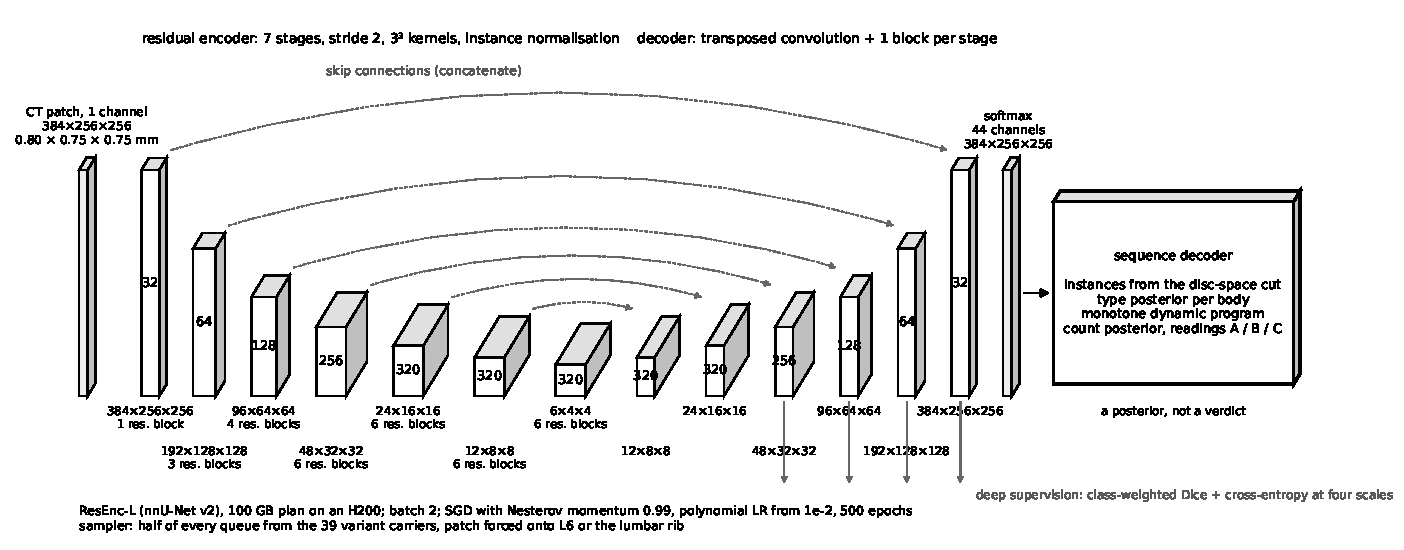
\includegraphics[width=\linewidth]{figs/fig_architecture.pdf}\\[4pt]
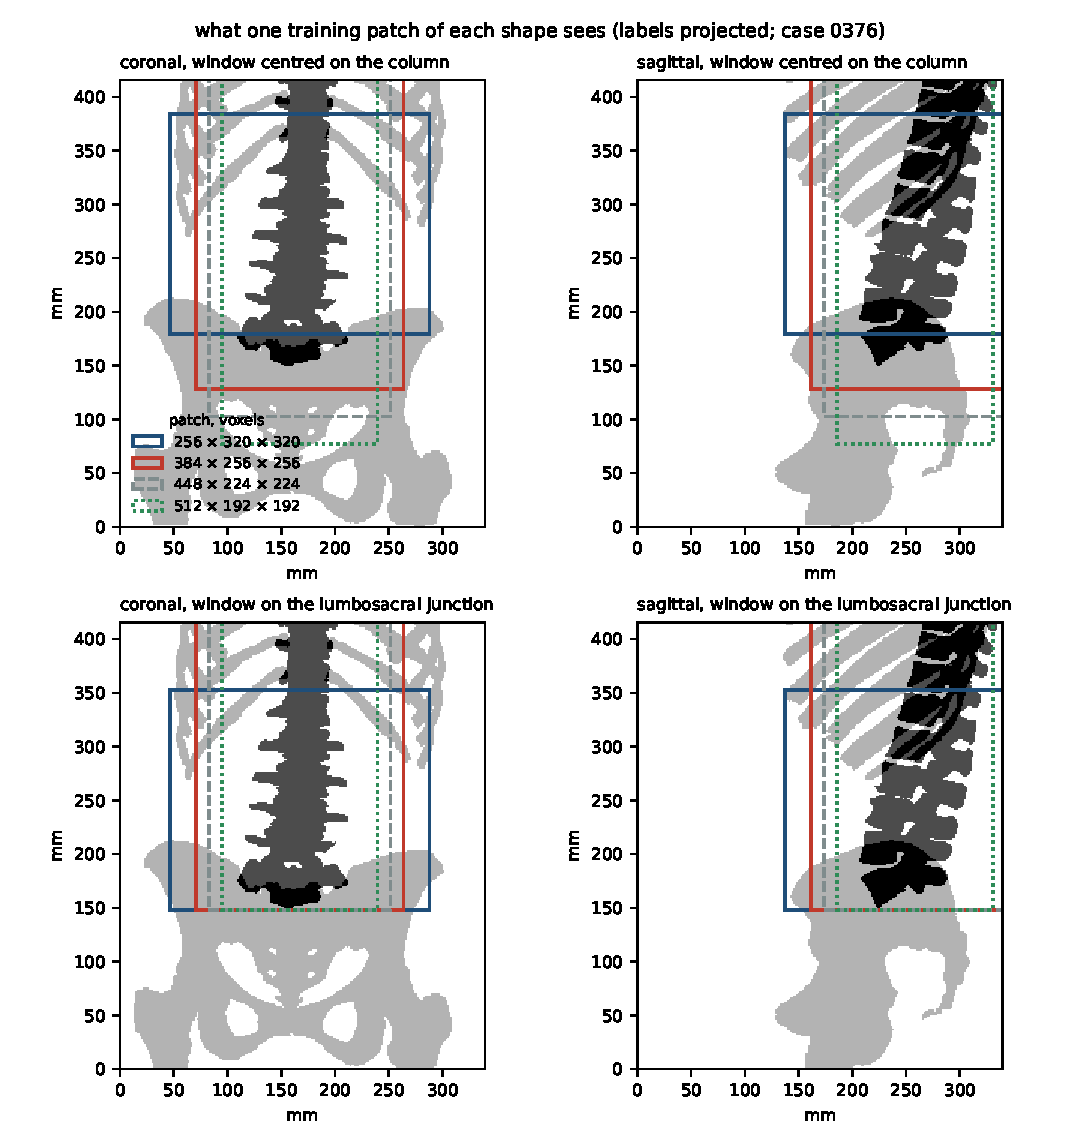
\includegraphics[width=0.85\linewidth]{figs/fig_patch_context_0376.pdf}\\[4pt]
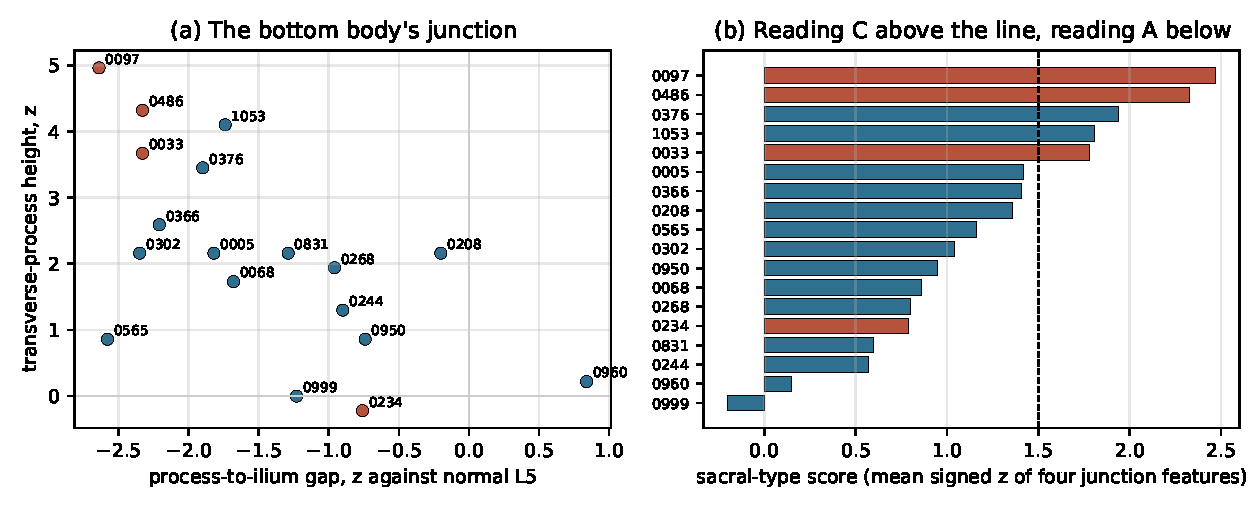
\includegraphics[width=\linewidth]{figs/six_lumbar_readings.pdf}
\end{document}
